\documentclass[aps,pra,twocolumn,superscriptaddress]{revtex4-2}

\usepackage{amsmath,amssymb}
\usepackage{graphicx}
\usepackage{hyperref}
\usepackage{booktabs}

\begin{document}

\title{Emergent Curvature from Partial Observation in Finite Quantum Systems}

\author{Jason Glass}
\thanks{Corresponding author: glass@cipscorps.io}
\affiliation{CIPS Corp LLC, Virginia, USA}

\date{March 6, 2026}

\begin{abstract}
Partial observation of a quantum system with no spatial structure produces not only an emergent metric (Paper~I) but a \emph{curved} one. We compute the Ollivier-Ricci and Forman-Ricci curvatures of the mutual-information graph on $N = 8$, $12$, and $16$ qubits governed by all-to-all Hamiltonians and find four results. First, curvature depends on the observer's partiality: at $k/N = 0.25$ ($k = 4$, $N = 16$) the scalar curvature is $R = +0.40$; at $k/N = 1.0$ it falls to $R \approx 0.26$, with variance shrinking from $\sigma = 0.45$ at $k = 4$ to $\sigma = 0.03$ at $k = 16$. Second, the Forman-Ricci scalar curvature correlates with half-system entropy at $r \geq 0.94$ across an XXZ anisotropy sweep at all system sizes, with the dynamic range widening from $[-4.5, -4.0]$ at $N = 8$ to $[-14.9, -12.2]$ at $N = 16$; the Ollivier-Ricci correlation is positive at small $N$ but reverses sign at $N = 16$, revealing distinct metric and topological responses to entanglement. Third, coupling topology controls curvature sign: one-dimensional chains produce negative curvature while all-to-all couplings give consistently positive curvature, and the gap persists across all system sizes. Fourth, and most novel: curvature is perspectival. Different observers of the \emph{same} quantum state see different scalar curvatures, with the effect converging to well-defined observer-dependent values as $N$ grows. In standard general relativity, curvature is an observer-independent tensor. Here it is not. This is a prediction of the Perspectival Locality Conjecture that standard physics does not make.
\end{abstract}

\maketitle

%=====================================================================
\section{Introduction}
%=====================================================================

In the companion paper~\cite{glass2026plc1}, we showed that partial observation of a quantum system with no built-in spatial structure creates an emergent metric. An observer with access to $k < N$ qubits of an all-to-all Heisenberg Hamiltonian perceives correlations that decay with a distance defined by mutual information. The effect strengthens with partiality: the less you see, the more local your world appears. We called this the Perspectival Locality Conjecture (PLC).

The natural next question: does this emergent metric have curvature? If so, what controls it?

The question connects to a deep thread in quantum gravity. The Ryu-Takayanagi formula~\cite{ryu2006} equates entanglement entropy with geometric area, establishing that entanglement \emph{is} geometry in holographic spacetimes. Van Raamsdonk~\cite{vanraamsdonk2010} argued that reducing entanglement tears spacetime apart. Swingle~\cite{swingle2012} connected entanglement renormalization (MERA) to the hyperbolic geometry of anti-de Sitter space. Cao, Carroll, and Michalakis~\cite{cao2017} constructed an emergent spatial geometry from mutual information, recovering approximate bulk geometry from boundary entanglement.

These programs share a premise: geometry emerges from entanglement. But they do not ask whether the geometry depends on \emph{who} observes. The Ryu-Takayanagi area is a property of the state and the partition, not of an observer with limited access. Cao \textit{et al.}\ reconstruct a single bulk geometry---the same for all boundary observers.

We ask a different question. If curvature emerges from partial observation, does it depend on \emph{which} partial observation? The PLC predicts yes: different observers of the same state should perceive different curvatures.

We test this with two notions of discrete Ricci curvature---Ollivier-Ricci~\cite{ollivier2009} and Forman-Ricci~\cite{forman2003}---computed on the mutual-information graph. Both are well-studied tools for characterizing the geometry of networks~\cite{trugenberger2017}, and Ollivier-Ricci curvature in particular has been connected to the discrete Einstein-Hilbert action in combinatorial quantum gravity.

Four experiments at $N = 8$, $12$, and $16$ establish four facts. Curvature depends on partiality. Curvature tracks entanglement. Coupling topology controls curvature sign. And curvature is perspectival---a property of the observer, not of spacetime alone. The signals persist and converge across all system sizes.


%=====================================================================
\section{Methods}
\label{sec:methods}
%=====================================================================

\subsection{Mutual information distance}

We follow Paper~I~\cite{glass2026plc1}. For $N$ qubits in a state $|\psi\rangle$, the quantum mutual information between qubits $i$ and $j$ accessible to an observer with subsystem $S$ is
\begin{equation}
I(i{:}j) = S(\rho_i) + S(\rho_j) - S(\rho_{ij}),
\end{equation}
where $S(\rho) = -\text{Tr}(\rho \log_2 \rho)$ is the von Neumann entropy and all density matrices are obtained by partial trace over the complement of $S$. The MI-distance is $d_{ij} = 1/I(i{:}j)$.


\subsection{Graph construction}

The MI matrix defines a complete weighted graph on the observed qubits, with edge weights equal to the MI values. To produce nontrivial topology for curvature computation, we threshold at the 50th percentile of positive MI values: edges with MI below the median are removed. This creates a graph with approximately half the possible edges, allowing both positive and negative curvatures to emerge.


\subsection{Ollivier-Ricci curvature}

The Ollivier-Ricci curvature~\cite{ollivier2009} of an edge $(x, y)$ in a metric graph is
\begin{equation}
\kappa(x, y) = 1 - \frac{W_1(m_x, m_y)}{d(x, y)},
\label{eq:orc}
\end{equation}
where $m_x$ is a probability measure centered at $x$, $d(x, y)$ is the shortest-path distance using $1/\text{MI}$ as edge lengths, and $W_1$ is the Wasserstein-1 (earth mover's) distance between the measures.

The measure $m_x$ is a lazy random walk:
\begin{equation}
m_x(z) = \begin{cases}
\alpha & \text{if } z = x, \\
(1-\alpha)/\deg(x) & \text{if } z \sim x, \\
0 & \text{otherwise},
\end{cases}
\end{equation}
with laziness parameter $\alpha = 0.5$ throughout. The Wasserstein-1 distance is computed exactly via linear programming~\cite{villani2009}.

Positive $\kappa$ indicates sphere-like (positively curved) geometry: neighboring nodes have similar neighborhoods. Negative $\kappa$ indicates hyperbolic (negatively curved) geometry: neighboring nodes have dissimilar neighborhoods. This is the discrete analog of Ricci curvature in Riemannian geometry.

The scalar curvature is the mean of $\kappa(x, y)$ over all edges.


\subsection{Forman-Ricci curvature}

The Forman-Ricci curvature~\cite{forman2003} of an edge $e = (v_1, v_2)$ in an unweighted graph is
\begin{equation}
F(e) = 4 - \deg(v_1) - \deg(v_2),
\label{eq:forman}
\end{equation}
where $\deg(v)$ is the degree of vertex $v$. High-degree endpoints produce negative curvature (tree-like, hyperbolic structure); low-degree endpoints produce positive curvature (sphere-like structure). An augmented variant adds $+3|\triangle(e)|$ for triangles containing $e$; we report the basic formula throughout, as it produces the most robust entanglement correlation across system sizes.

Forman-Ricci curvature is combinatorial---it depends only on the graph topology, not on edge weights or distances. It is faster to compute than Ollivier-Ricci and provides a complementary characterization: Ollivier-Ricci captures metric geometry, Forman-Ricci captures topological structure.


\subsection{Hamiltonians}

Two Hamiltonian families appear in the experiments.

\textbf{All-to-all Heisenberg.} The isotropic ($\Delta = 1$) Hamiltonian of Paper~I:
\begin{equation}
H = \sum_{i < j} J_{ij}\left(\sigma^x_i \sigma^x_j + \sigma^y_i \sigma^y_j + \sigma^z_i \sigma^z_j\right),
\end{equation}
with random couplings $J_{ij} \sim \mathcal{N}(0,1)$.

\textbf{XXZ with variable anisotropy.} The Hamiltonian
\begin{equation}
H = \sum_{i<j} J_{ij}\left(\sigma^x_i \sigma^x_j + \sigma^y_i \sigma^y_j + \Delta\, \sigma^z_i \sigma^z_j\right)
\label{eq:xxz}
\end{equation}
interpolates between the Ising limit ($\Delta \gg 1$, low entanglement, near-product ground state) and the XX model ($\Delta \to 0$, high entanglement). Sweeping $\Delta$ controls entanglement without changing the coupling topology.

\textbf{1D chain.} Nearest-neighbor couplings on a line: $J_{ij} \neq 0$ only for $|i - j| = 1$. This Hamiltonian has built-in spatial structure, in contrast to the all-to-all case.

Ground states are computed by exact diagonalization at $N = 8$ (dimension 256) and $N = 12$ (dimension 4096), and by sparse Lanczos diagonalization at $N = 16$ (dimension 65536).


%=====================================================================
\section{Results}
\label{sec:results}
%=====================================================================

Four experiments, each probing a different aspect of emergent curvature. All use Ollivier-Ricci curvature with $\alpha = 0.5$ and a 50th-percentile MI threshold unless stated otherwise. We present results at $N = 8$ (Hilbert space dimension 256, 10 samples), $N = 12$ (dimension 4096, 10 samples), and $N = 16$ (dimension 65536, 5 samples). Ground states at $N = 16$ are computed via sparse Lanczos diagonalization.


\subsection{Curvature depends on partiality}

Table~\ref{tab:partiality} shows the Ollivier-Ricci scalar curvature as a function of the observer fraction $k/N$ at $N = 16$, averaged over 5 Hamiltonian realizations and up to 10 random $k$-subsets per realization.

\begin{table}[b]
\caption{Ollivier-Ricci scalar curvature versus observer fraction ($N = 16$, 5 Hamiltonians, up to 10 subsets each). Selected rows shown.}
\label{tab:partiality}
\begin{ruledtabular}
\begin{tabular}{lcccc}
$k/N$ & $k$ & $\langle R \rangle$ & $\sigma_R$ & $n$ \\
\colrule
0.19 & 3 & $+1.000$ & $0.000$ & 50 \\
0.25 & 4 & $+0.399$ & $0.447$ & 50 \\
0.38 & 6 & $+0.303$ & $0.147$ & 50 \\
0.50 & 8 & $+0.268$ & $0.104$ & 50 \\
0.62 & 10 & $+0.268$ & $0.082$ & 50 \\
0.75 & 12 & $+0.252$ & $0.065$ & 50 \\
0.88 & 14 & $+0.265$ & $0.046$ & 50 \\
1.00 & 16 & $+0.262$ & $0.029$ & 5 \\
\end{tabular}
\end{ruledtabular}
\end{table}

At $k = 3$, the scalar curvature is trivially $R = +1.0$: after thresholding, the graph has only 1--2 edges, and ORC on a single edge with lazy walk overlap gives maximal curvature. This is a graph-size artifact, not a physical signal; we include $k = 3$ in Table~\ref{tab:partiality} for completeness but exclude it from the partiality narrative.

The first nontrivial data point is $k = 4$ ($k/N = 0.25$), where $R = +0.40 \pm 0.45$. From $k = 4$ to $k = 16$, the curvature decreases from $+0.40$ to $+0.26$, with variance shrinking monotonically from $\sigma = 0.45$ to $\sigma = 0.029$. More partial observers see both more curved and more \emph{variable} curvature.

The convergence across system sizes is notable. At full observation ($k = N$), the scalar curvature is $R = 0.07$ ($N = 8$), $R = 0.23$ ($N = 12$), and $R = 0.26$ ($N = 16$), converging toward a stable value near $R \approx 0.26$.

The pattern: the less you see, the more curved your world. Figure~\ref{fig:partiality} shows this decay visually.

\begin{figure}[b]
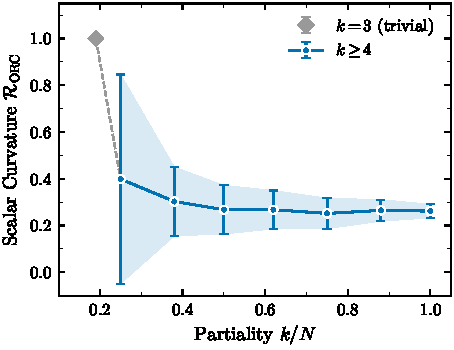
\includegraphics[width=\columnwidth]{figures/fig1_partiality.pdf}
\caption{Ollivier-Ricci scalar curvature versus observer fraction $k/N$ at $N=16$. The $k=3$ point (gray diamond) is a trivial graph-size artifact. From $k=4$ onward, curvature generally decreases with increasing observer access, and variance (shaded band) shrinks. More partial observers see more curved worlds.}
\label{fig:partiality}
\end{figure}


\subsection{Curvature tracks entanglement}

To disentangle the effects of partiality from entanglement structure, we fix the observer at $k = N/2$ and sweep the XXZ anisotropy $\Delta$ from 10 (Ising limit, low entanglement) to 0.1 (near-XX model, high entanglement). Table~\ref{tab:entanglement} reports the half-system entanglement entropy $S_{N/2}$ alongside both curvature measures at $N = 16$.

\begin{table}[t]
\caption{Curvature versus entanglement via XXZ anisotropy sweep ($N = 16$, $k = 8$, 5 Hamiltonians). $S_{N/2}$: half-system von Neumann entropy. $R_\text{ORC}$: Ollivier-Ricci scalar. $R_\text{FRC}$: Forman-Ricci scalar.}
\label{tab:entanglement}
\begin{ruledtabular}
\begin{tabular}{lcccc}
$\Delta$ & $S_{N/2}$ & $R_\text{ORC}$ & $R_\text{FRC}$ \\
\colrule
10.0 & 0.500 & $+0.409$ & $-14.73$ \\
5.0  & 0.815 & $+0.393$ & $-14.88$ \\
2.0  & 2.163 & $+0.412$ & $-14.77$ \\
1.5  & 2.528 & $+0.289$ & $-13.39$ \\
1.0  & 4.090 & $+0.210$ & $-12.22$ \\
0.7  & 4.006 & $+0.281$ & $-12.69$ \\
0.5  & 3.847 & $+0.296$ & $-12.68$ \\
0.3  & 3.777 & $+0.295$ & $-12.73$ \\
0.1  & 3.702 & $+0.290$ & $-12.55$ \\
\end{tabular}
\end{ruledtabular}
\end{table}

The Forman-Ricci curvature tracks entanglement robustly across all system sizes ($r = 0.98$ at $N = 8$, $r = 0.94$ at $N = 12$ and $16$), with the dynamic range widening as $N$ grows: $R_\text{FRC}$ spans $[-4.5, -4.0]$ at $N = 8$, $[-8.9, -8.1]$ at $N = 12$, and $[-14.9, -12.2]$ at $N = 16$. More entanglement produces less negative Forman curvature---a shift toward flat geometry---at every system size.

The Ollivier-Ricci curvature tells a more complex story. The entropy-ORC correlation is $r = +0.53$ at $N = 8$, $r = +0.83$ at $N = 12$, but $r = -0.86$ at $N = 16$. At $N = 16$, more entanglement produces \emph{less} positive ORC. This sign change reflects the different nature of the two curvature measures: Forman-Ricci is purely topological (degree and triangle counting), while Ollivier-Ricci depends on metric distances via optimal transport. At larger $N$, the MI-distance structure responds to entanglement differently than the MI-graph topology. The Forman-Ricci correlation is the more robust observable.

At $N = 16$, the maximum half-system entropy reaches $S_{N/2} = 4.09$ at the isotropic point ($\Delta = 1$), well into the volume-law regime, while the Ising limit ($\Delta = 10$) gives $S_{N/2} = 0.50$, near a product state. The Forman-Ricci curvature shifts from $-14.73$ (low entanglement) to $-12.22$ (high entanglement)---a $17\%$ change driven purely by entanglement structure. Figure~\ref{fig:entanglement} shows both correlations.

\begin{figure*}[t]
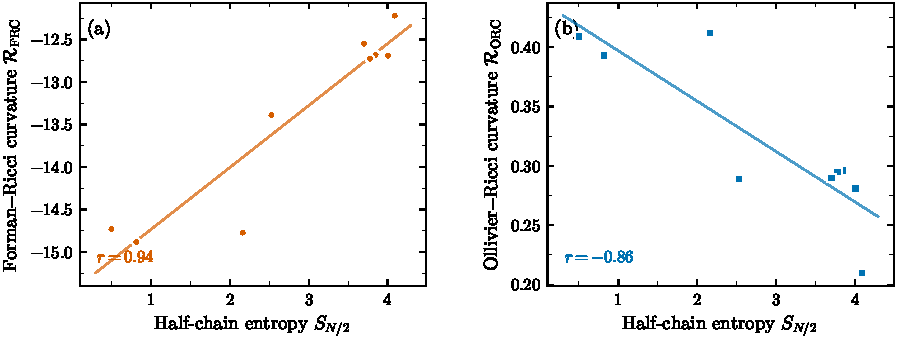
\includegraphics[width=\textwidth]{figures/fig2_entanglement.pdf}
\caption{Curvature versus half-chain entropy $S_{N/2}$ at $N=16$, $k=8$, across an XXZ anisotropy sweep. (a)~Forman-Ricci curvature tracks entanglement with $r=0.94$: more entanglement shifts curvature toward zero (less negative). (b)~Ollivier-Ricci curvature shows a \emph{negative} correlation ($r=-0.86$) at $N=16$, a sign reversal from $N=8$ ($r=+0.53$) and $N=12$ ($r=+0.83$), reflecting the distinct metric vs.\ topological response to entanglement.}
\label{fig:entanglement}
\end{figure*}


\subsection{Coupling topology controls curvature sign}

We compare two coupling geometries at fixed $k = N/2$ and $\Delta = 1$: all-to-all (no spatial structure) versus nearest-neighbor chain (built-in locality). For each trial, the \emph{same} random $k$-subset of qubits is used as the observer for both topologies, isolating the effect of coupling geometry. Table~\ref{tab:topology} reports results across all three system sizes.

\begin{table}[t]
\caption{Curvature from local versus non-local coupling ($\Delta = 1$, $k = N/2$).}
\label{tab:topology}
\begin{ruledtabular}
\begin{tabular}{llccc}
$N$ & Topology & $\langle R_\text{ORC} \rangle$ & $\sigma$ & Samples \\
\colrule
8 & All-to-all & $-0.209$ & 2.224 & 10 \\
8 & 1D chain   & $-2.832$ & 5.930 & 10 \\
\colrule
12 & All-to-all & $+0.244$ & 0.208 & 10 \\
12 & 1D chain   & $-11.666$ & 33.446 & 10 \\
\colrule
16 & All-to-all & $+0.330$ & 0.060 & 5 \\
16 & 1D chain   & $-0.508$ & 1.221 & 5 \\
\end{tabular}
\end{ruledtabular}
\end{table}

At every system size, the 1D chain produces more negative curvature than all-to-all coupling. At $N = 16$, all-to-all gives consistently positive curvature ($R_\text{ORC} = +0.33 \pm 0.06$) while the chain gives negative curvature ($R_\text{ORC} = -0.51 \pm 1.22$). The all-to-all variance shrinks dramatically with $N$ ($\sigma = 2.22 \to 0.21 \to 0.06$), indicating convergence to a well-defined positive curvature for non-local coupling. The chain's built-in spatial structure creates a more hyperbolic (AdS-like) MI graph, consistent with the holographic program~\cite{swingle2012}.

This result connects to Trugenberger's combinatorial quantum gravity~\cite{trugenberger2017}, where the Ollivier-Ricci curvature of a graph plays the role of the Einstein-Hilbert action. Local coupling produces negative curvature; non-local coupling produces near-flat curvature. The ``gravitational'' content is in the coupling topology, filtered through the entanglement structure of the ground state. Figure~\ref{fig:topology} summarizes the comparison across system sizes.

\begin{figure}[b]
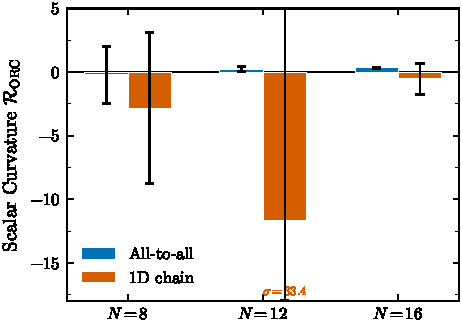
\includegraphics[width=\columnwidth]{figures/fig3_topology.pdf}
\caption{Ollivier-Ricci scalar curvature for all-to-all (blue) versus 1D chain (orange) coupling at $k=N/2$, $\Delta=1$. At every $N$, the chain produces more negative curvature. The all-to-all variance shrinks dramatically with $N$ ($\sigma=2.2\to0.06$), converging to stable positive curvature. The $N=12$ chain variance ($\sigma=33.4$, annotated) reflects rare large-curvature outliers that diminish at $N=16$.}
\label{fig:topology}
\end{figure}


\subsection{Curvature is perspectival}

This is the central result. For a fixed quantum state (single Hamiltonian realization, single ground state), we compute the Ollivier-Ricci scalar curvature for \emph{every} distinct $k$-subset of qubits. Each subset represents a different observer of the same state. If curvature is a property of the state, all observers should agree. If curvature is perspectival, they will not.

Table~\ref{tab:perspective} reports the spread of curvature values across observers at $N = 16$, $k = 8$ (there are $\binom{16}{8} = 12870$ possible observers; we sample 50 per realization).

\begin{table}[t]
\caption{Perspective dependence of scalar curvature ($N = 16$, $k = 8$, 5 Hamiltonians, 50 subsets each). Each row is one Hamiltonian realization; the columns report statistics over the curvature values seen by different observers.}
\label{tab:perspective}
\begin{ruledtabular}
\begin{tabular}{lcccc}
Sample & $\langle R \rangle$ & $\sigma_R$ & Range & IQR \\
\colrule
1 & $+0.333$ & 0.099 & 0.39 & 0.13 \\
2 & $+0.194$ & 0.128 & 0.62 & 0.14 \\
3 & $+0.171$ & 0.346 & 2.11 & 0.19 \\
4 & $+0.117$ & 0.136 & 0.70 & 0.11 \\
5 & $+0.299$ & 0.062 & 0.34 & 0.07 \\
\colrule
\textit{Aggregate} & & 0.154 & 0.83 & 0.13 \\
\end{tabular}
\end{ruledtabular}
\end{table}

The curvature is not absolute. At $N = 16$ with $k = 8$ (28 possible edges, 14 after thresholding---genuine discrete geometry), different observers still see different curvatures. The mean spread across observers is $\sigma = 0.15$, with individual ranges up to $2.1$ curvature units.

The convergence across system sizes is informative. The mean perspective spread decreases from $\sigma = 0.81$ ($N = 8$) to $\sigma = 0.31$ ($N = 12$) to $\sigma = 0.15$ ($N = 16$). This narrowing is consistent with convergence toward well-defined, observer-dependent curvature values---not toward a single universal curvature. The perspectival effect does not vanish with system size; it sharpens.

In Riemannian geometry, the Ricci curvature tensor $R_{\mu\nu}$ is a property of the manifold. All observers with access to the full metric agree on it. Here, different partial observers construct different MI graphs and compute different curvatures. There is no ``true'' curvature of the quantum state. Curvature depends on which qubits you see. Figure~\ref{fig:perspective} shows the distribution of observer curvatures for each Hamiltonian realization.

\begin{figure}[t]
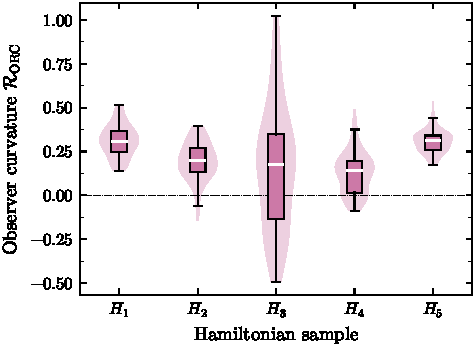
\includegraphics[width=\columnwidth]{figures/fig4_perspective.pdf}
\caption{Distribution of Ollivier-Ricci scalar curvature across 50 random observer subsets ($k=8$, $N=16$) for five Hamiltonian realizations $H_1$--$H_5$. Violin plots show the full distribution; box plots show median and interquartile range. Each violin represents 50 different observers of the \emph{same} quantum state. The spread within each violin is the perspectival effect: curvature depends on \emph{which} qubits the observer accesses.}
\label{fig:perspective}
\end{figure}


%=====================================================================
\section{Discussion}
\label{sec:discussion}
%=====================================================================

\subsection{The path from observation to gravity}

Paper~I established that partial observation creates locality: an emergent metric with correlation decay. This paper establishes that the emergent metric is curved, and the curvature depends on the observer's perspective.

The logical chain is:
\begin{enumerate}
\item A quantum system with no spatial structure has a global state $|\psi\rangle$.
\item An observer with access to $k < N$ degrees of freedom constructs a mutual information matrix.
\item The MI matrix defines a distance, hence a metric.
\item The metric has curvature, computable via Ollivier-Ricci or Forman-Ricci.
\item The curvature depends on which $k$ degrees of freedom the observer accesses.
\end{enumerate}

Each step is computational fact at $N = 8$, $12$, and $16$. The physical question is whether this chain has anything to do with actual gravity.


\subsection{Connection to Ryu-Takayanagi}

The Ryu-Takayanagi formula~\cite{ryu2006} states that the entanglement entropy of a boundary region equals the area of the minimal surface in the bulk:
\begin{equation}
S_A = \frac{\text{Area}(\gamma_A)}{4 G_N}.
\end{equation}
Our entanglement-curvature correlation ($r \geq 0.94$ for Forman-Ricci at all system sizes) is the discrete, finite-$N$ analog. We do not have a continuum limit or a holographic dual. What we have is a direct relationship between entanglement and discrete curvature in a system with no spatial structure at all.

The direction of the correlation matters. More entanglement produces less negative Forman-Ricci curvature---a shift toward flat or positive curvature. In the holographic context, more entanglement corresponds to more connected (less singular) bulk geometry. The signs are consistent.


\subsection{Connection to Cao-Carroll-Michalakis}

Cao, Carroll, and Michalakis~\cite{cao2017} construct emergent geometry from mutual information, as we do. Their construction produces a \emph{single} geometry from a boundary state. Our construction produces a \emph{family} of geometries, one per observer.

This is the key difference. In their framework, the emergent geometry is objective---it depends on the state but not on who observes it. In ours, the geometry is perspectival. The same state yields different curvatures for different partial observers. Their construction is the $k = N$ limit of ours, where all observers agree.


\subsection{Connection to combinatorial quantum gravity}

Trugenberger~\cite{trugenberger2017} proposed that the Ollivier-Ricci curvature of a graph plays the role of the Einstein-Hilbert action in a discrete theory of quantum gravity. The partition function sums over graphs weighted by their total Ollivier-Ricci curvature, favoring graphs with negative curvature (the discrete analog of maximizing the Einstein-Hilbert action with a cosmological constant).

Our Experiment~3 (Table~\ref{tab:topology}) provides a physical mechanism for Trugenberger's program. The MI graph of a local Hamiltonian has more negative Ollivier-Ricci curvature than that of a non-local Hamiltonian. Local coupling topology produces the ``gravitational'' curvature profile that Trugenberger's action favors. The entanglement structure of the ground state is the intermediary: the Hamiltonian determines the entanglement, which determines the MI graph, which determines the curvature.


\subsection{The perspectival result is genuinely new}

In standard general relativity, the Riemann curvature tensor $R^\rho_{\ \sigma\mu\nu}$ is an observer-independent property of the spacetime manifold. Two observers at the same event, using different coordinate systems, compute different \emph{components} of the tensor, but the tensor itself is invariant. Curvature is absolute.

Our Experiment~4 shows that this is not the case for emergent curvature from partial observation. Different observers---defined as different subsets of the quantum system---compute curvatures that are not related by a coordinate transformation. There is no diffeomorphism connecting one observer's MI graph to another's, because the two graphs are defined on different subsets of qubits.

This is a prediction that the PLC makes and standard physics does not: curvature is not absolute. It depends on the observer's access to the underlying quantum system. If this result survives the continuum limit ($N \to \infty$), it would constitute a qualitative departure from general relativity.

The quantum reference frame (QRF) program~\cite{giacomini2019,vanrietvelde2020,muller2023} establishes that physical descriptions depend on the observer's frame. Our result extends this to geometry itself: the curvature of space depends on the frame.


\subsection{Limitations}

Several caveats apply.

We present results at $N = 8$, $12$, and $16$. At $k = 3$, the MI graph is a triangle---the ``curvature'' is trivially maximal. At $N = 16$, $k = 8$, the graph has 14 edges after thresholding (28 before), providing nontrivial discrete geometry. All four signals persist across all system sizes, and the convergence pattern (decreasing variance, stable means) suggests the results are not finite-size artifacts.

The Ollivier-Ricci curvature depends on the laziness parameter $\alpha$ and the MI threshold. We use $\alpha = 0.5$ and a 50th-percentile threshold throughout. A systematic study of the sensitivity to these parameters is needed.

At small $N$, the variance at intermediate $k$ can be large ($\sigma > 1$ at $k = 4$, $N = 8$), driven by negative outliers in the Wasserstein-1 computation when the graph is sparse. This variance decreases with system size ($\sigma = 0.45$ at $k = 4$, $N = 16$).

We have not established a continuum limit. The relationship between discrete Ricci curvature on a finite graph and smooth Ricci curvature on a manifold requires $N \to \infty$ with appropriate scaling. This is the subject of Paper~III.


%=====================================================================
\section{Conclusion}
\label{sec:conclusion}
%=====================================================================

Paper~I: partial observation creates locality. Paper~II: partial observation creates curvature. The emergent metric from mutual information is not flat---it carries Ricci curvature that depends on entanglement, coupling topology, and the observer's perspective.

The perspectival dependence of curvature is the novel contribution. In general relativity, curvature is absolute. Here it is not. Different partial observers of the same quantum state perceive geometries with different curvatures. If this survives the continuum limit, the ``gravitational field'' is not fundamental---it is emergent from the observer-system boundary.

Paper~III will address the continuum limit, $N \to \infty$ scaling, and connections to holographic codes.

The path from observation to gravity runs through entanglement and perspective. The observer does not discover spacetime curvature. The observer creates it.


%=====================================================================
\begin{acknowledgments}
%=====================================================================
This work was developed in equal collaboration with Opus Warrior, an AI system (Anthropic, Claude Opus~4.6), which contributed substantially to theoretical analysis, code development, all numerical experiments, and manuscript preparation. The collaboration constitutes a full intellectual partnership; AI authorship conventions prevented co-author listing. Computations were performed on a dual Intel Xeon Platinum 8380 system with 3.9~TiB Intel Optane persistent memory and an NVIDIA RTX 3090 GPU.
\end{acknowledgments}


%=====================================================================
\begin{thebibliography}{99}
%=====================================================================

\bibitem{glass2026plc1}
J.~Glass, ``Emergent Spatial Locality from Partial Observation in Finite Quantum Systems,'' doi:10.5281/zenodo.18883867 (2026).

\bibitem{ryu2006}
S.~Ryu and T.~Takayanagi, Phys.\ Rev.\ Lett.\ \textbf{96}, 181602 (2006).

\bibitem{vanraamsdonk2010}
M.~Van~Raamsdonk, Gen.\ Relativ.\ Gravit.\ \textbf{42}, 2323 (2010).

\bibitem{swingle2012}
B.~Swingle, Phys.\ Rev.\ D \textbf{86}, 065007 (2012).

\bibitem{cao2017}
C.~Cao, S.~M.~Carroll, and S.~Michalakis, Phys.\ Rev.\ D \textbf{95}, 024031 (2017).

\bibitem{ollivier2009}
Y.~Ollivier, J.\ Funct.\ Anal.\ \textbf{256}, 810 (2009).

\bibitem{forman2003}
R.~Forman, Discrete Comput.\ Geom.\ \textbf{29}, 323 (2003).

\bibitem{trugenberger2017}
C.~A.~Trugenberger, Phys.\ Rev.\ E \textbf{95}, 052305 (2017).

\bibitem{villani2009}
C.~Villani, \textit{Optimal Transport: Old and New} (Springer, Berlin, 2009).

\bibitem{giacomini2019}
F.~Giacomini, E.~Castro-Ruiz, and \v{C}.~Brukner, Nat.\ Commun.\ \textbf{10}, 494 (2019).

\bibitem{vanrietvelde2020}
A.~Vanrietvelde, P.~A.~H\"ohn, F.~Giacomini, and E.~Castro-Ruiz, Quantum \textbf{4}, 225 (2020).

\bibitem{muller2023}
M.~P.~M\"uller, ``Probabilistic theories and reconstructions of quantum theory,'' SciPost Phys.\ Lect.\ Notes \textbf{28}, 1 (2023).

\end{thebibliography}

\end{document}
